\documentclass[a4paper, 12pt]{article}

%% placeholder komandai
\usepackage{color}
%%Graphics
\usepackage{graphicx}
%%PDF index
%\usepackage[bookmarks]{hyperref}

%% Lietuviški rašmenys, lietuviškų žodžių skirstymas į skiemenis, lietuviški kai kurio dokumento dalių pavadinimai.
\usepackage{polyglossia}
\setdefaultlanguage{lithuanian}

%%paraštes
\usepackage[margin = 2cm]{geometry}
%% pavojingos eilutes
\widowpenalty 1000
\clubpenalty 1000

\usepackage{setspace}
\onehalfspacing


%% Atitraukti pirmą pastraipą.
\usepackage{indentfirst}

%% komandos
\newcommand{\OK}{Oleg Koldun PS1}
\newcommand{\UC}{Ugnė Laima Čižiutė PS1}
\newcommand{\RK}{Rytis Karpuška PS1}
\newcommand{\DK}{Donatas Kučinskas PS1}
\newcommand{\KJ}{Karolis Jocevičius PS1}
\newcommand{\placeholder}{\textbf{\textsf{\textcolor{red}{\fbox{PLACEHOLDER}}}}}


%	instrukcija:
%	"%" 	- komentaras uz jo galima rasyti viska
%	"\" 	- sintaksinis elementas komandai atskirti
%	"{parametras}" 	- parametras komandai
%			pvz: \section{pavadinimas} - sukurs parafrafa su pavadinimu: "pavadinimas"
%	"\\" 	- perkelti teksta i nauja eilute
%	<dvigubas Enter> 	- nauja pastraipa
%	"\section{name} 	- parafrafas
%	"\subsection{name}"	- poskyris
%	"\newpage"	- naujas puslapis
%	
%	software:	instalinat xelatex, reikiamus paketus jis pats suinstalins bandant padaryti faila(~4GB)
%	make instruction: 	xelatex ReferatasZKS.tex
%---------------------------------------------------------
% 		Paveikslėlio įkėlimo pavyzdys:
%
%		\begin{figure}[h]
%		\centering
%		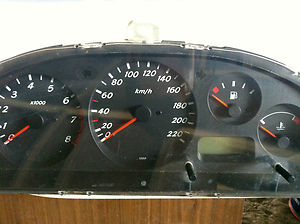
\includegraphics[width=0.8\textwidth]{images/almera.JPG}
%		\caption{Nissan Almera prietaisų skydelis}
%		\label{overflow}
%		\end{figure}
%
% Jei prireiktų atributų, žr.: http://en.wikibooks.org/wiki/LaTeX/Importing_Graphics

\begin{document}



	%%titulinis


	\begin{titlepage}

		\begin{center}
	
			\large {Vilniaus universitetas
	
					Matematikos ir Informatikos fakultetas}
			
			\vspace*{\fill}
	
		\textsc{\Huge Pastebėti esamų interfeisų (ne)patogumai} \\[0.5cm]
%%		{\Large placeholder}
	
		\vspace{3cm}
	
			\begin{flushright}
				\begin{minipage}{0.35\textwidth}
				{\large Darbą atliko:} \\
					\KJ \\
					\UC \\
					\OK \\
					\DK \\
					\RK
				\end{minipage}
			\end{flushright}
	
			\vspace{\fill}
	
			{\Large Vilnius, \the\year}
			
		\end{center}
	\end{titlepage}
	
	%%anotacija

\section*{Anotacija}
	
		\textbf{Darbą atliko:}
		
		
		%%%%%%%%%%%%%%%%%%%%%%%%%%%%%%%%%%%%%
		\textbf{\KJ}
		\begin{flushleft}
		\hspace*{1.5cm}
		Kontaktai:
			karolis.jocevicius@gmail.com
		\\
		\hspace*{1.5cm}
		Indėlis: Nissan Almera laikrodžio nustatymas, GMail kortelės 
		\end{flushleft}
		%%%%%%%%%%%%%%%%%%%%%%%%%%%%%%%%%%%%%
		
		\textbf{\UC}
		\begin{flushleft}
		\hspace*{1.5cm}
		Kontaktai: 
			ugne.ciziute@gmail.com
		\\
		\hspace*{1.5cm}
		Indėlis: USB jungtis, Mikrobangų krosnelė
		\end{flushleft}
		%%%%%%%%%%%%%%%%%%%%%%%%%%%%%%%%%%%%%
		
		\textbf{\OK}
		\begin{flushleft}
		\hspace*{1.5cm}
		Kontaktai: 
			okoldun@gmail.com 
		\\
		\hspace*{1.5cm}
		Indėlis: Mobili 15min.lt versija, Microsoft Comamnd Prompt
		\end{flushleft}
		%%%%%%%%%%%%%%%%%%%%%%%%%%%%%%%%%%%%%

		\textbf{\DK}
		\begin{flushleft}
		\hspace*{1.5cm}
		Kontaktai: 
			donce.lt@gmail.com 
		\\
		\hspace*{1.5cm}
		Indėlis: Bankomatų ekranai, Numatytoji paveikslėlių peržiūra Windows 8 sistemoje
		\end{flushleft}
		%%%%%%%%%%%%%%%%%%%%%%%%%%%%%%%%%%%%%
		
		\textbf{\RK}
		\begin{flushleft}
		\hspace*{1.5cm}
		Kontaktai: 
			jauleris@gmail.com
		\\
		\hspace*{1.5cm}
		Indėlis: Google pagrindinis puslapis, Android skambučio nutraukimas
		\end{flushleft}
	\newpage{}	
	
	
	\tableofcontents
	\newpage
	%%skyriai		



% nuo cia pradedam rasyti
	
\section{pavyzdžiai}
	\subsection{USB jungtis}
		\textbf{Tikslas -}
		prijungti USB įrenginį prie kompiuterio.

		\textbf{Priemonės -} 
		USB įrenginys ir kompiuteris su laisvu USB lizdu.

		\textbf{Rezultatas -}
		nepavyko prijungti USB įrenginio iš pirmo karto.

		\textbf{Panaudojamumo projektavimo principai, aktualūs šioje situacijoje:}
		\begin{itemize}
		\item Nuspėjamumas – naudotojas iškarto mato, kad USB kištukas turi būti kišamas į USB lizdą, tačiau jis nežino, kuria puse jį reikia kišti.
		\item Sintezavimas – pusė, kuria kišamas USB kištukas kiekviename įrenginyje gali skirtis.
		\item Atvaizdis - ant USB kištuko yra nurodyta jo viršutinė dalis, tačiau labai neaiškiai. USB lizdas sufleruoja, kuria puse reikia kišti kištuką, tačiau tai nurodanti žymė būna per daug maža, kad naudotojas ją pastebėtų.
		\end{itemize}

		\textbf{Pamąstymai -}
		Projektuotojai padarė teisingai nurodydami kuria puse reikia kišti USB kištuką, tačiau jie nepagalvojo, kad jų užuominos yra per daug menkos ir retas, kas jas pastebės. 
		Geriausias sprendimas būtų spalvos - ausinių/mikrofono kištukai bei jų lizdai yra nuspalvinti atitinkamomis spalvomis, kad naudotojai jų nesupainiotų, ta pati idėja galėtų būti pritaikyta ir USB jungčiai.
		
		\begin{figure}[h]
		\centering
		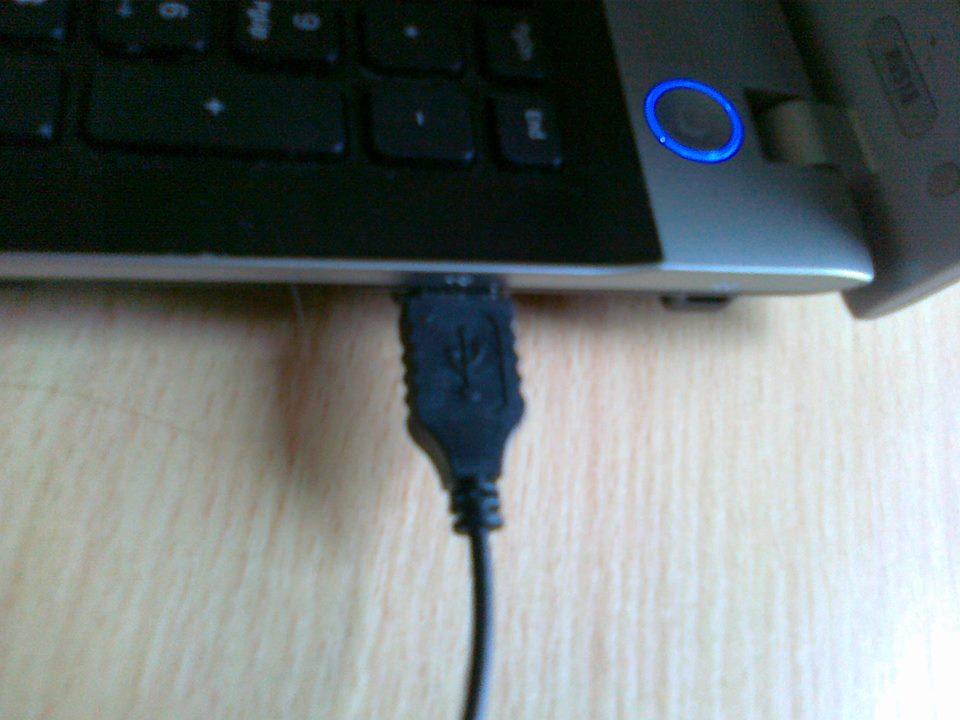
\includegraphics[width=0.8\textwidth]{images/usb.jpg}
		\caption{USB lizdas}
		\label{overflow}
		\end{figure}
	\subsection{Mikrobangų krosnelė}
		\textbf{Tikslas -}
		pasišildyti maistą

		\textbf{Priemonės -} 
		laikmatis ir temperatūrą nustatanti rankenėlė

		\textbf{Rezultatas -}
		maistas pašilo per nurodytą laiką

		\textbf{Panaudojamumo projektavimo principai, aktualūs šioje situacijoje:}
		\begin{itemize}
		\item Nuspėjamumas – naudotojas iškarto mato įrenginio naudojimo principą.	
		\item Sintezavimas – nustačius laikmatį naudotojas iškart pastebi įrenginio būsenos pasikeitimą.
		\item Apibendrinimas – seno tipo bei pigios mikrobangų krosnelės valdomos tuo pačiu principu.
		\end{itemize}

		\textbf{Pamąstymai -}
		Ši mikrobangų krosnelė yra pilnai nuspėjama, todėl naudotojas gali greitai, be jokio vargo ja pasinaudoti. 
		Daugumai naujo tipo mikrobangų krosnelių reikia naudojimosi instrukcijos, dėl jų įvairiapusio funkcionalumo, tačiau dažniausiai naudotojui tereikia greitai pasišildyti maistą.	

		\begin{figure}[h]
		\centering
		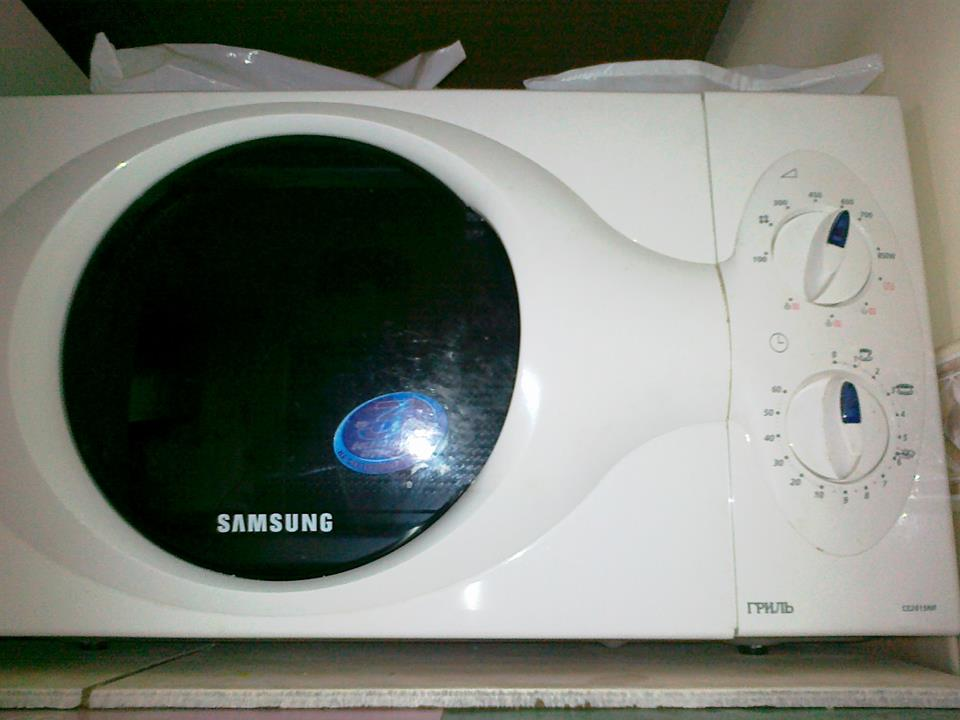
\includegraphics[width=0.8\textwidth]{images/mikrobange.jpg}
		\caption{Mikrobangų krosnelė}
		\label{overflow}
		\end{figure}		
	\subsection{Microsoft Comamnd Prompt}
		\textbf{Tikslas -}
		Patogiai naudotis keliais komandiniais langais.
		
		\textbf{Priemonės -}
		Kompiuteris, klaviatūra, pelė.
		
		\textbf{Rezultatas -}
		Kompiuteris įvykdo jam įvestas komandas.	
		
		\textbf{Atvaizdis -}
		Langas riboto dydžio (neįmanoma nustatyti reikiamo vartotojui dydžio).

		\textbf{Panaudojamumo projektavimo principai, aktualūs šioje situacijoje:}
		\begin{itemize}
		\item Nuspėjamumas - naudotojas iškarto mato kai jo įvestos komandos vykdomos.
		\item Sintezavimas - įvedus komandą arba tekstus vartotojas iškarto mato rezultatus arba komandos vykdymo pradžią.
		\end{itemize}

		\textbf{Pamąstymai -}
		Sklandžiai veikiantis produktas, bet nėra pilnai pritaikomas vartotojo patogumui.
		\begin{figure}[h]
		\centering
		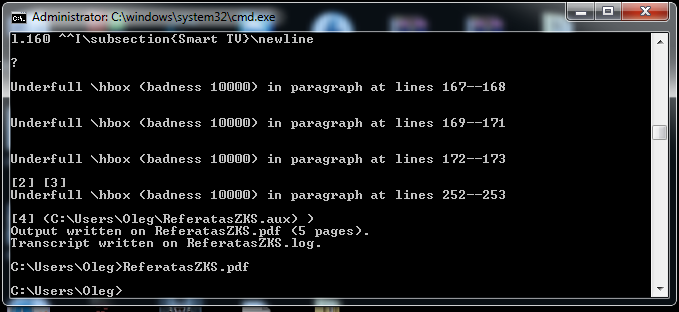
\includegraphics[width=0.8\textwidth]{images/command-prompt.png}
		\caption{Maksimalus leidžiamas plotis}
		\label{overflow}
		\end{figure}
	\subsection{Mobili 15min.lt versija}	
		\textbf{Tikslas -}
		Peržiūrėti staipsnius.

		\textbf{Priemonės -}
		Išmanusis telefonas.

		\textbf{Rezultatas -}
		Peržiūrėtas straipsnis.

		\textbf{Atvaizdis -}
		Straipsniai lengvai prieinami, bet grįžtant atgal iš straipsnio, vėl permetama į puslapio pradžią.
		
		\textbf{Panaudojamumo projektavimo principai, aktualūs šioje situacijoje:}
		\begin{itemize}
		\item Nuspėjamumas - nenuspėjama, nes naudotojas įpratęs, kad paspaudus "Back" mygtuką, jį grąžins į tą pačią vietą.
		\item Sintezavimas - vartotojas iš karto pasiekia jam norimą straipsnį, bet kaskart sekančio straipsnio reikia ieškoti iš naujo.	
		\end{itemize}

		\textbf{Pamąstymai -}:
		Vartotojams būtų paprasčiau naudotis, jeigu staipsnių archyvas butų išskaidytas į smulkesnius puslapius.

	\subsection{Nissan Almera laikrodžio nustatymas}
		\textbf{Tikslas -}
		Nustatyti teisingą laiką automobilio laikrodyje.

		\textbf{Priemonės -}
		Mygtukas spidometro skydelyje, kilometražo/laikrodžio ekranas.

		\textbf{Rezutatas -}
		Nustatytas teisingas laikas.

		\textbf{Atvaizdis -}
		Mygtukas skirtas laiko nustatymui atrodantis lygiai taip pat kaip ir kilometražo atstatymo mygtukas,
		ekranas kilometražo bei laiko rodymui.
		
		\textbf{Panaudojamumo projektavimo principai, aktualūs šioje situacijoje:}
		\begin{itemize}
		\item Nuspėjamumas - nenuspėjama, nes nėra jokių ženklų rodančių mygtuko paskirt į ar veikimo principą.
		\item Sintezavimas - vartotojas gali nustatyti laiką, tačiau nėra aišku kaip tą padaryti, be
		to nustatinėti laiką vienu mygtuku - nepatogu bei užtrunka per daug laiko.
		\end{itemize}

		\textbf{Pamąstymai -}
		Vartotojui būtų paprasčiau, jei laikrodis būtų nustatinėjamas dvejais mygtukais (minutės, valandos)
		bei būtų aiški mygtuko paskirtis.

		%% Paveikslėlio įkėlimo pavyzdys
		\begin{figure}[h]
		\centering
		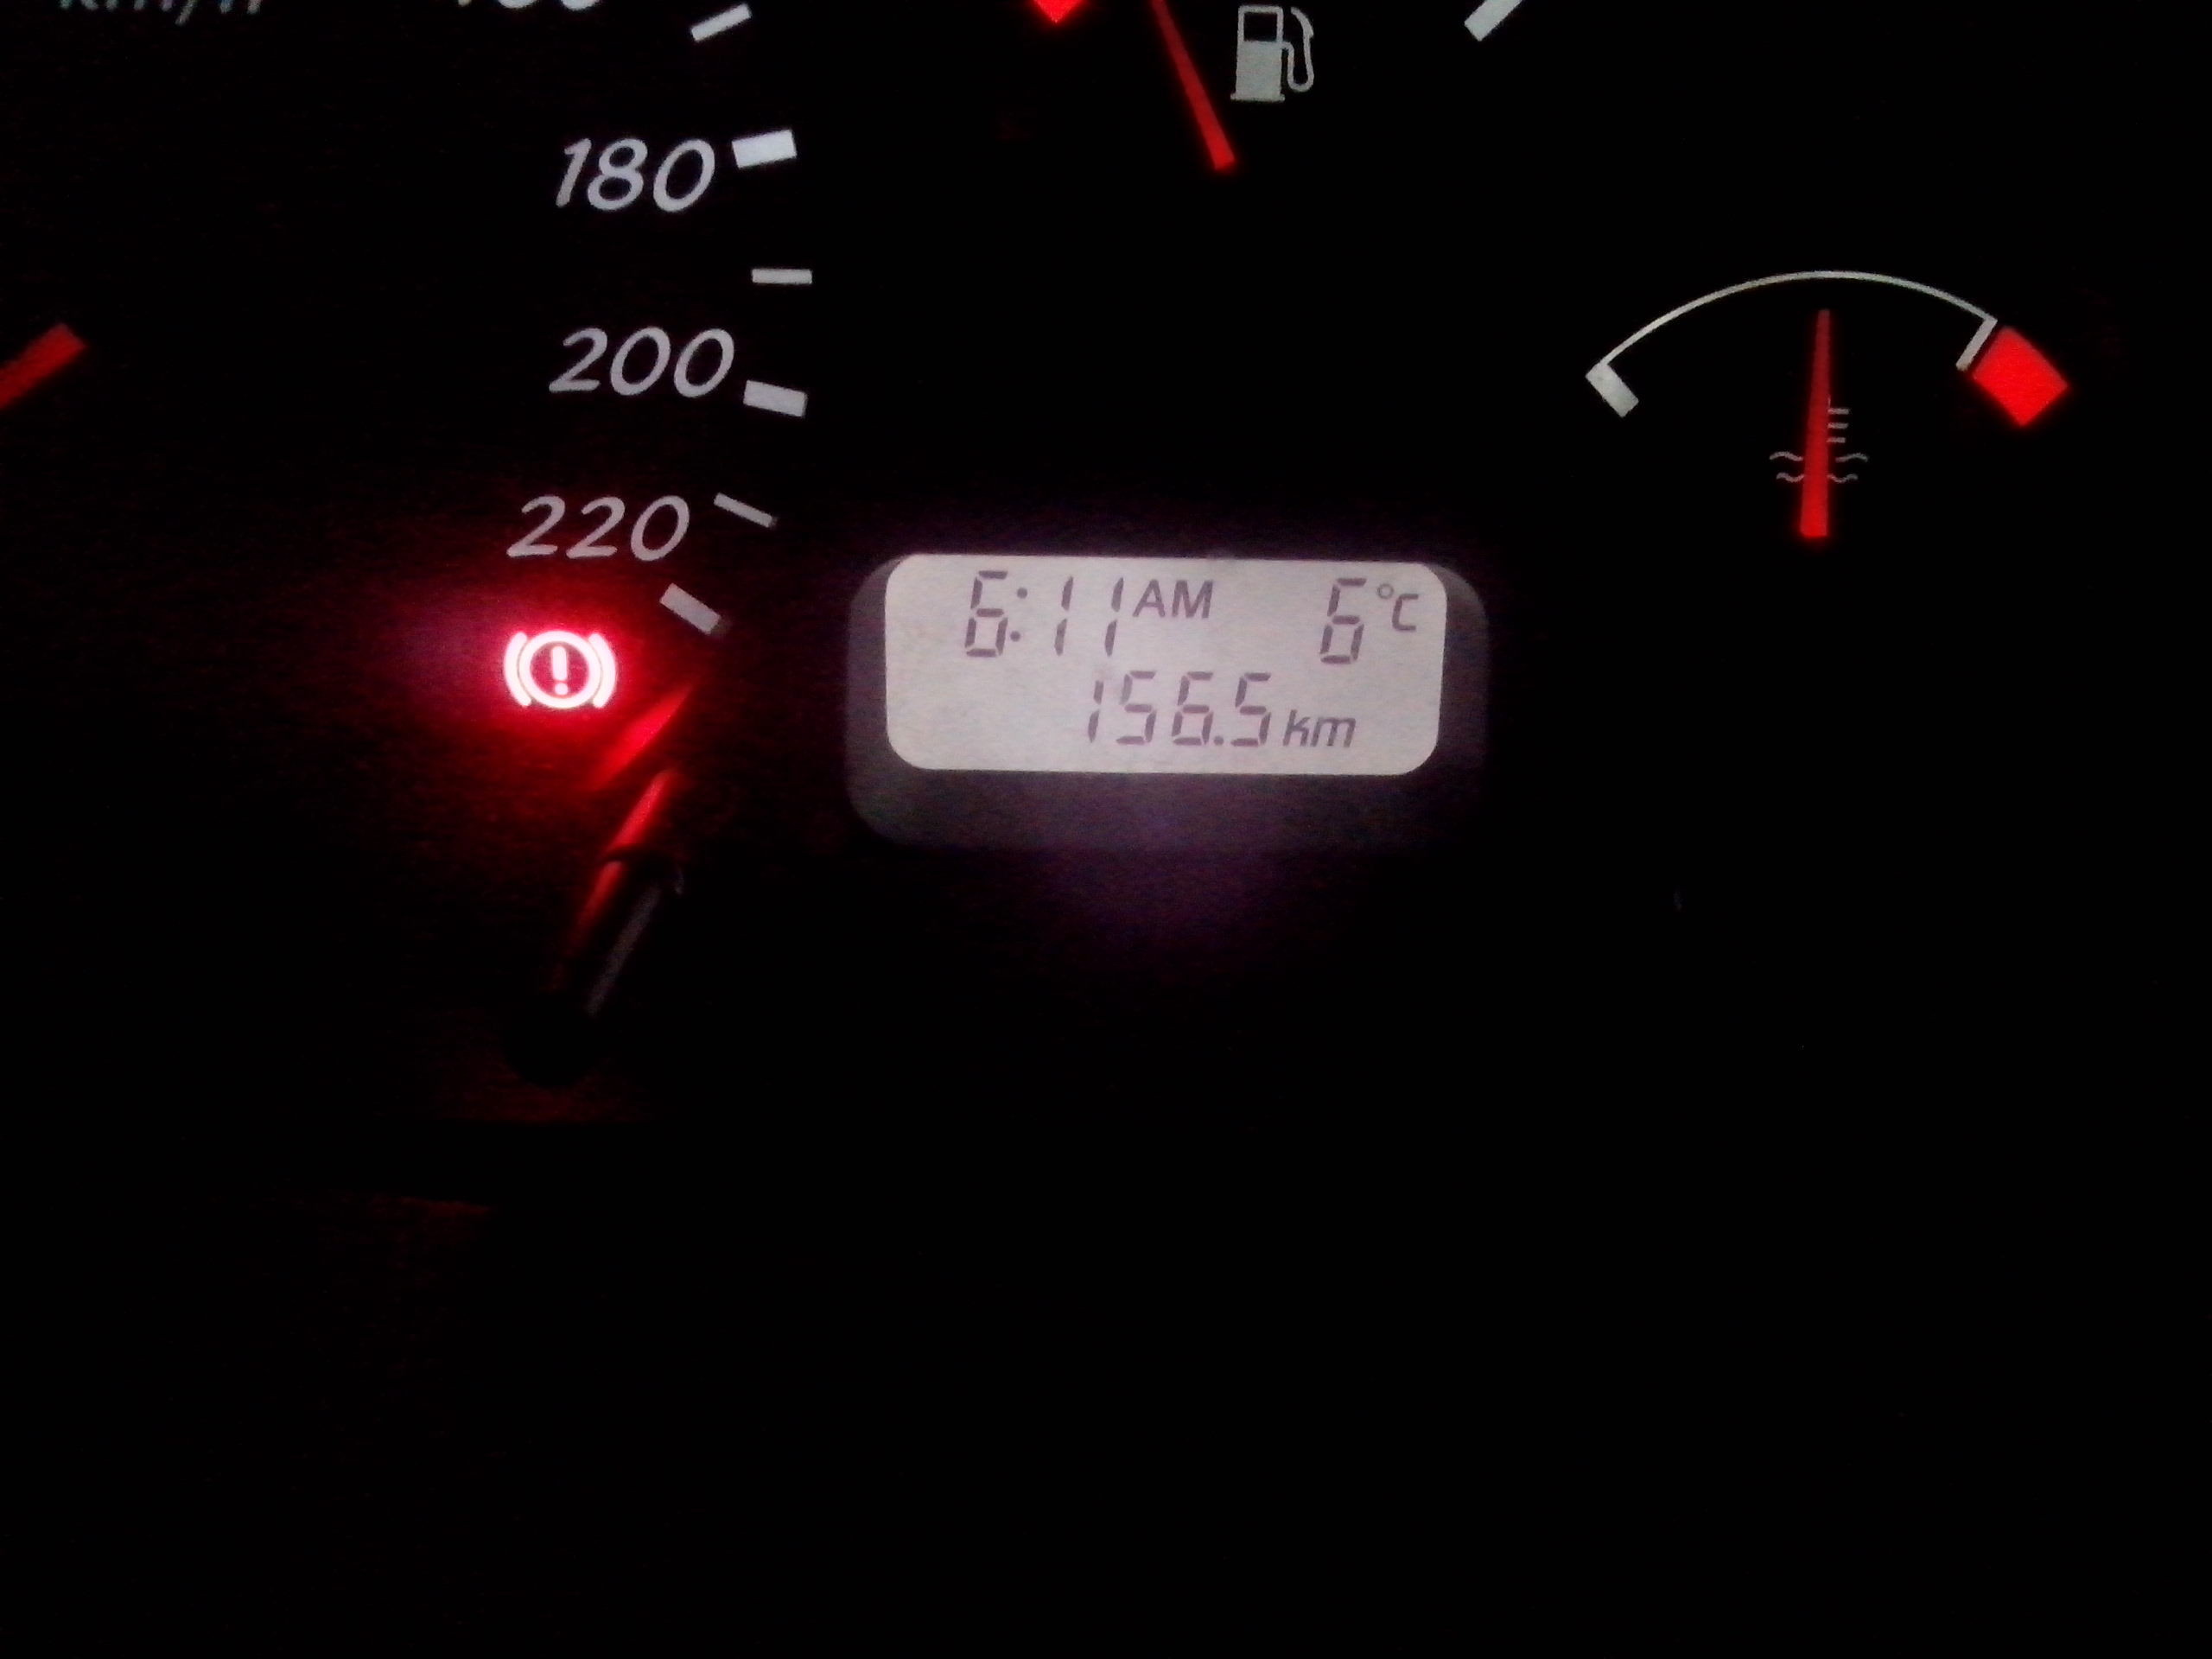
\includegraphics[width=0.8\textwidth]{images/almera.jpg}
		\caption{Nissan Almera prietaisų skydelis}
		\label{almera}
		\end{figure}
		
	\subsection{GMail kortelės}
		\textbf{Tikslas -}
		Peržiūrėti kortelėse esančius laiškus

		\textbf{Priemonės -}
		Gmail gautųjų laiškų langas su kortelėmis
		
		\textbf{Rezultatas -}
		Peržiūrėti kortelėse surūšiuoti laiškai.

		\textbf{Atvaizdis -}
		Kortelių juosta virš laiškų sąrašo leidžia pasirinkti rodomą kortelę.
		
		\textbf{Panaudojamumo projektavimo principai, aktualūs šioje situacijoje:}
		\begin{itemize}
		\item Nuspėjamumas - nuspėjama, nes kortelės yra standartinis ir įprastas vartotojo sąsajos elementas.
		\item Sintezavimas - vartotojas gali peržiūrėti surūšiuotus laiškus ir matyti neperskaitytų laišku kiekį kortelėje, tačiau peržiūrėjus laišką grąžinamas pagrindinis laiškų vaizdas, o kortelių juostoje pradingsta neperskaitytų laiškų lankytoje kortelėje kiekis.	
		\end{itemize}

		\textbf{Pamąstymai -}
		Vartotojui būtų patogiau, jei peržiūrėjus laišką esantį kortelėje būtų grįžtama į prieš tai lankytą kortelę.
		Taip pat nereikėtų išvalyti neperskaitytų kortelės laiškų rodymo.

		\begin{figure}[h]
		\centering
		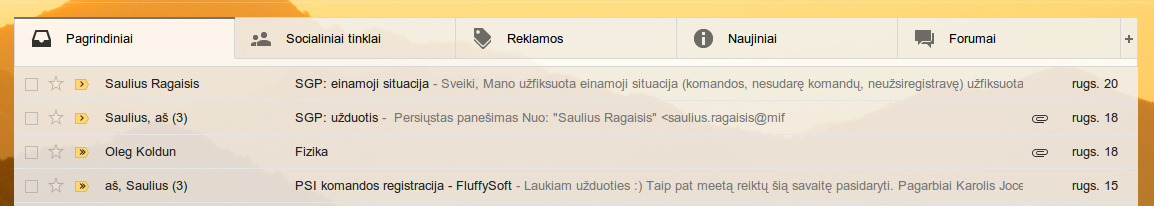
\includegraphics[width=0.8\textwidth]{images/korteles.png}
		\caption{GMail kortelės}
		\label{korteles}
		\end{figure}

	\subsection{Google pagrindinis puslapis}
		\textbf{Tikslas -}
		Rasti sau dominančią informaciją.

		\textbf{Priemonės -}
		Tekstinė paieška.
		
		\textbf{Rezultatas -}
		Internete rastos informacijos pateikimas svetainių sąrašo, atitinkančių tekstinę užklausą, principu.\\
		
		\textbf{Atvaizdis -}
		Įprastas teksto įvedimo laukelis.

		\textbf{Panaudojamumo projektavimo principai, aktualūs šioje situacijoje:}
		\begin{itemize}
		\item Lankstumas - Google sąsaja turi labai mažai elementų (paieškos funkciją galima atlikti pasinaudojus tik teksto įvedimo laukeliu), bet funkcionalumas nėra apribojamas.
		Pavyzdžiui ieškodami youtube vaizdelio, įvykdę paiešką su susijusia užklausa, mums bus pateikiami youtube video pasiūlymai.
		Taip pat adreso/vietos paieška pateikia žemėlapį, kai kurie skaičiavimai atliekami už mus.
		Nespėjus suvesti visos užklausos, iškarto matome pasiūlymus, kaip galėtume užbaigti savo paiešką - stiprinama dialogo iniciatyva.
		Priedo netyčia padarius klaidą, yra pasiūlomi gramatinių klaidų pataisymai - vykdomas užduočių perkelimas.
		\item Robastiškumas - Vartotojui atsidarius google paieškos puslapį, rodomas pagrindinis sąsajos elementas tiesiai per vidurį, pačioje matomiausioje vietoje - įgyvendinamas matomumo principas.
		Taip pat sąsaja yra labai dinamiška, pradėjus vesti, iškarto matome sąrašą svetainių, atrinktą pagal tai ką jau suvedėme (net ir tuo atveju, jeigu užklausa dar kol kas nebuvo suvesta iki galo).
		Taigi įvykdomas sistemos atsako principas.
		\end{itemize}

		\textbf{Pamąstymai -}
		lankstumas ir robastiškumas google sąsajose išsprendžiamas, pateikiant labai intuityvią sąsają, o išmokstamumas sprendžiamas padarant šią sąsąja itin paprastą naudoti.
		Pasinaudoti google, turbūt yra netgi lengviau, negu paklausti draugo to paties klausimo.

		\begin{figure}[h]
		\centering
		
\includegraphics[width=0.8\textwidth]{images/google.jpg}
		\caption{Google pagrindinis ekranas}
		\label{korteles}
		\end{figure}

	\subsection{Android skambučio nutraukimas}
		\textbf{Tikslas -}
		Pranešti kodėl vartotojas negali atsiliepti.

		\textbf{Priemonės -}
		Specialus, išanksto numatytų žinučių sąrašas, skirtų išsiųsti dar skambučio metu.

		\textbf{Rezultatas -}
		Nutraukiamas skambutis ir pranešama kodėl vartotojas negalėjo atsiliepti.

		\textbf{Atvaizdis -}
		Brūkštelėjus apačioje išvažiuojantis žinučių sąrašas su iš anksto užpildytu tekstu.

		\textbf{Panaudojamumo projektavimo principai, aktualūs šioje situacijoje:}
		\begin{itemize}
		\item Išmokstamumas - pasinaudojus šiuo funkcionalumu netgi vieną kartą, be papildomų pastangų yra aišku kaip jį panaudoti dar kartą.
		Šis sąsajos elementas yra gerai integruotas į bendrą android aplinką, nes "ištraukiamų" papildomų nustatymų, ar kitų elementų android sistemoje galima sutikti dažnai.
		Tad įgyvendinami nuspėjamumo, atpažįstamumo, bei darnos principai.
		\item Robastiškumas - Turint omenyje vartojimo aplinką, mums yra būtina minimizuoti veiksmų, reikalingų pasiekti šiam tikslui, skaičių.
		Todėl užduotis tampa sudėtingesnė.
		Laimei šis sąsajos elementas yra atliekamas dviem prisilietimais prie ekrano - tad sąsaja gerai tinkama užduoties atlikimui.
		Taip pat pasirinkus norimą žinutę iš sąrašo, sistema automatiškai nutraukia skambutį, todėl galime teigti, kad sistemos atsako principas irgi yra įgyvendintas sėkmingai.
		\end{itemize}

		\textbf{Pamąstymai -}
		Sąsajos elementas ištiesų suprojektuotas patogiai, ir naudojimas yra intuityvus.
		Mano manymu patobulėti galima tik pastiprinus matomumo principą. 

		\begin{figure}[h]
		\centering
		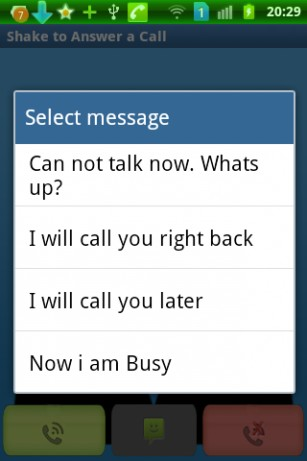
\includegraphics[width=0.4\textwidth]{images/android.jpg}
		\caption{Android skambučio nutraukimo žinutės}
		\label{korteles}
		\end{figure}
		\newpage %% kompiliuojant be new page paveiksliukas atsiranda neteisingoje vietoje
	
	\subsection{Bankomatų ekranai}
		\textbf{Tikslas -}
		Leisti vartotojui patikrinti savo banko sąskaitos pinigų likutį, išsiimti grynųjų pinigų.

		\textbf{Priemonės -}
		Ekranas, skirtas rodyti vartotojo banko informaciją.
		Šonuose - mygtukai, kurių funkcijos rašomos ekrane, mygtukų šonuose.

		\textbf{Rezultatas -}
		Vartotojas gauna prieigą prie savo banko sąskaitos, gali į ją įnešti ir iš jos išsiimti pinigų.

		\textbf{Panaudojamumo projektavimo principai, aktualūs šioje situacijoje:}\\
		Jeigu į ekraną nešviečia saulė, naudotis visai patogu.
		Tačiau jeigu diena saulėta, šviesa nuo ekrano labai atsispindi, todėl įžiūrėti tekstą yra gan sunku.

		\textbf{Pamąstymai -}
		Vartotojui, ypač turinčiam nusilpusį regėjimą, naudotis tokiu interfeisu gali būti sunku.
		Reikėtų kaip nors pagerinti ekrano matumumą - pavyzdžiui, visus bankomatus laikyti patalpų viduje arba įrengti budelę.
		Tokiu būdu bankomato ekranas būtų apsaugotas nuo saulės atspindžių ir naudotis šiuo interfeisu taptų kur kas lengviau.

		\begin{figure}[h]
		\centering
		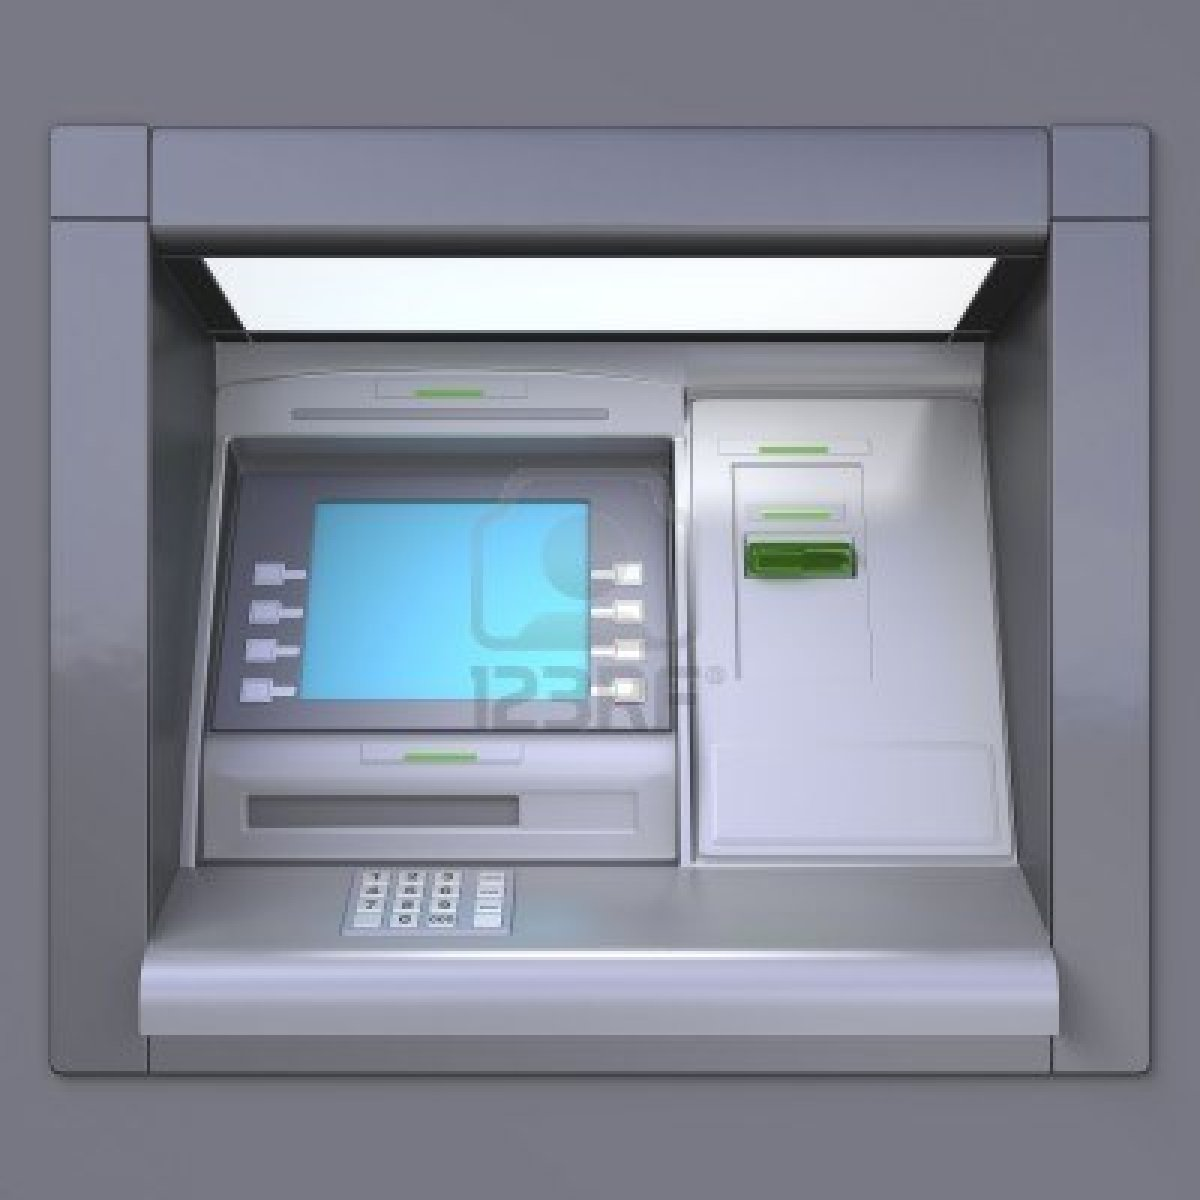
\includegraphics[width=0.8\textwidth]{images/atm.jpg}
		\caption{Bankomatas}
		\label{bankomatas}
		\end{figure}
		\newpage %% kompiliuojant be new page paveiksliukas atsiranda neteisingoje vietoje
		
	\subsection{Numatytoji paveikslėlių peržiūra Windows 8 sistemoje}
		\textbf{Tikslas -}
		Pavaizduoti vartotojo atidarytą paveikslėlį ekrane.
		
		\textbf{Priemonės -}
		Paveiksliuko failas, kurį norima atidaryti; monitorius, kuriame bus pavaizduotas paveiksliukas.

		\textbf{Rezultatas -}
		Monitoriaus ekrane rodomas norimas paveiksliukas.

		\textbf{Panaudojamumo projektavimo principai, aktualūs šioje situacijoje:}
		\begin{itemize}
		\item Nuspėjamumas - Interfeiso nuspėjamumas yra prastas - atidaromas paveikslėlis rodomas per visą ekraną, negalima pakeisti rodomo paveikslėlio įprastais būdais (pvz. rodyklių klavišais).
		\item Sintezavimas - Vartotojo norimas atidaryti paveiksliukas atsidarė, tačiau jis užima visą ekraną - norint pasiekti kokią nors informaciją iš darbastalio, reikia grįžti į darbastalį, o dėl to reikia atlikti papildomų veiksmų bei uždaryti paveiksliuką.
		\end{itemize}

		\textbf{Pamąstymai -}
		Tokia paveiksliuko peržiūra labai nepatogi, jeigu norima peržiūrėti kelis paveikslėlius arba atliekant kelis darbus vienu metu.
		Tai ypač nepatogu vartotojams, kurie yra pratę prie įprastų paveikliukų peržiūros programų, kurios paveiksliuko per visą ekraną iš karto neatidaro (arba bent leidžia sumažinti).

		\begin{figure}[h]
		\centering
		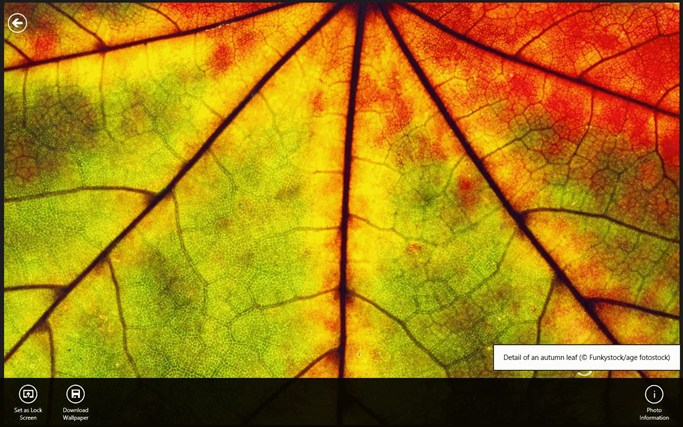
\includegraphics[width=0.8\textwidth]{images/win8.jpg}
		\caption{Windows8 paveksliukų peržiūros programa}
		\label{win8}
		\end{figure}

\end{document}
